\documentclass[conference, onecolumn]{IEEEtran}
\usepackage{cite}
\usepackage{amsmath,amssymb,amsfonts}
\usepackage{algorithmic}
\usepackage{graphicx, subfig}
\usepackage{textcomp}
\usepackage{xcolor}
\usepackage{listings}
\usepackage{hyperref}
\usepackage{float}

\def\BibTeX{{\rm B\kern-.05em{\sc i\kern-.025em b}\kern-.08em T\kern-.1667em\lower.7ex\hbox{E}\kern-.125emX}}

\begin{document}

\title{Manual ADS-B Communication Protocol Implementation on the ADALM-PLUTO Using GNURadio}

\author{
    \IEEEauthorblockN{Alan Manuel Loreto Cornídez}
    \IEEEauthorblockA{\textit{College of Electrical and Computer Engineering} \\
    \textit{The University of Arizona}\\
    Tucson, Arizona \\
    aloretocornidez@arizona.edu}
\and
    \IEEEauthorblockN{Jeremy Sharp}
    \IEEEauthorblockA{\textit{College of Electrical and Computer Engineering} \\
    \textit{The University of Arizona}\\
    Tucson, Arizona \\
    jeremysharp@arizona.edu}
}

\maketitle

\begin{IEEEkeywords}
  Software Defined Radio, ADS-B, GNURadio
\end{IEEEkeywords}

\begin{abstract}
  The ADALM-PLUTO is a Software Defined Radio that has the capability to transmit and receive signals. Using the Pluto, we transmitted and received Automatic Dependent Surveillance-Broadcast (ADS-B) signals that are centered about 1090MHz. Multiple implementations were tested such as a MATLAB example, as well as an out of tree module for ADS-B communication for use in GNURadio. A custom implementation of ADS-B communication was made in GNURadio as well as a program written in C/C++ to decode received packets in and retrieve latitude and longitude of an aircraft that transmits the ADS-B signal.
\end{abstract}



\section{Introduction}
The most common method for aircraft to report their system state involves the use of the Automatic Dependent Surveillance-Broadcast (ADS-B) transmission method. An open transmission method used to broadcast an aircraft's position, enabling the ability to track the aircraft. Throughout the Spring 2024 semester, we have worked with the ADA Pluto Software Defined Radio (SDR) to receive and transmit signals in multiple ranges of frequency bands. We have implemented pre-made signal processing blocks in GNURadio signal flow graphs and then implemented them on the ADA Pluto for applications such as FM Radio and AM radio. Our project would like to work on solving the "1090 MHz Riddle". What is the 1090 MHz Riddle you may ask? For many Software Defined Radio (SDR) enthusiasts, being able to capture, decode, interpret, and transmit ADS-B signals involves an understanding of how signals are are manipulated in the RF spectrum, both for transmission and modulation. In our particular case, we would like to implement the use of the 1090 MHz frequency band to communicate with public aircraft information. We have found pre-made GNURadio block that implement ADS-B communication protocols, however, we would like to explore a custom implementation using only a GNURadio signal flow graph and the QT GUI elements. After implementing a simple receiver and transmitter, we would like to expand the project scope to receive real ADS-B signals transmitted by aircraft.

\section{ADS-B Introduction}
The ADS-B protocol is a used to transmit information about an aircraft while the aircraft is in flight. The ADS-B can be used to transfer information about the aircraft's location, direction, and air speed. This protocol is used by aircraft in many places around the world such as the United States, Canada, Europe, and Australia. The United States made it a requirement to fly with ADS-B equipped aircraft in January 2020. 

\section{ADS-B Frame Structure}
Let us break down the frame structure of an ADS-B packet so that we can decode the information contained within. 

An ADS-B packet contains 112 bits. The packet contains 5 main parts. 5 bits are used for the downlink format of the aircraft, 3 bits are used to relay transponder capability information. 24 bits are used to transmit the ICAO aircraft address. 56 bits are used to transmit an extended squitter message. 5 bits are used to for a type code. Finally, the last 24 bits are used as an error check for the integrity of the packet using a cyclic redundancy check. As you can see in \autoref{fig:ads-b-bits}, provided by \cite{sun1090mhz}, the total amount of bits that are used in a ADS-B packer is 112. In addition to the use of the 112 bits in the message, there is also a 16 bit preamble used for frame synchronization.

% This is the table from https://mode-s.org/decode/content/ads-b/1-basics.html where the writer talks about the ads-b packet structure.
\begin{figure}
\begin{center}
\begin{tabular}{ | c | c | c | c | }
  Bit & No. Bits & Abbreviation & Information \\ 
  1–5 & 5 & DF & Downlink Format \\
  6–8 & 3 & CA & Transponder capability \\
  9–32 & 24 & ICAO & ICAO aircraft address \\
  33–88 & 56 & ME & Message, squitter \\
  (33–37) & (5) & (TC) & (Type code) \\
  89–112 & 24 & PI & Parity/Interrogator ID
\end{tabular}
\end{center}
\caption{A breakdown of an ADS-B packet.}\label{fig:ads-b-bits}
\end{figure}

%% Implementation
\section{Implementation}
Transmissions for ADS-B signals are made in the 1090 MHz frequency band which is within the capabilities of the ADALM-PLUTO, as such, the Pluto was used in our implementation. We wanted to have the best chances of implementing a successful solution for for both receiving and transmitting data, we decided to design and make custom antennas for the project. After making our custom antennas, we wanted to do some initial testing with an MVP to make sure that data transfer was successful on the Pluto, because of this, we attempted to make two minimum viable products (MVPs) using different approaches. The first approach involved the use of an ADS-B example provided by Mathworks in Matlab. The second MVP was the use of a GNURadio out of tree module that contains ADS-B framing, demodulation, and decoding blocks. After these two attempts were made, we created custom signal flow graphs that checked for an ADS-B frame preamble at the correct frequencies. More information about the implementations can be found below. Results for the complete implementation can be found in the Results section of the report.

%% Custom Antenna Design
\subsection{Custom Antenna Design}
In order to give the best possible chance of receiving 1090MHz signals we had to use a better antenna than the one provided in the PlutoSDR kit. The included antennas in the PlutoSDR kit have a very flat frequency response over the entire range of the SDR, this makes them a decent choice for the vast majority of signals out there, however they generally do not have the best performance for low signal strengths, requiring the user to increase the gain, thus magnifying the background noise. To work around this, we decided to build a customized antenna in order to improve the ability of the SDR to receive 1090MHz signals.

After browsing antenna designs that are popular within the ADS-B hobbyist community, we settled on what is known as the 4 radial spider antenna.
This design is based upon the common half wavelength dipole antenna, but with 4 legs of the antenna being ground, this has the effect in the far field of improving the off axis radiation pattern in the XZ and YZ planes, while rejecting signals emanating from below, thus reducing overall background noise.
This antenna, would give us better performance, while still having an extremely low part cost of five pieces of copper wire, and a single female SMA connector.

Before constructing the antenna, we performed some quick calculations in order to determine the lengths of the copper wire required.
We know that a full wavelength of 1090MHz is 27.
5cm, and that since it is based on a dipole, the total length of the two elements should be $\frac{1}{2}$ wavelength, thus 13.
75cm, and with each element being the same length, we know that each element should be $\frac{1}{4}$ wavelength or 6.
88cm long. In the process of fabrication, we were not exactly sure how the lengths of the elements would be measured after being soldered to the SMA connector, we then decided to cut each copper wire at 7.5cm, then trim them down afterwards while using a vector network analyzer to check reflections.

\begin{figure}
  \begin{center}
    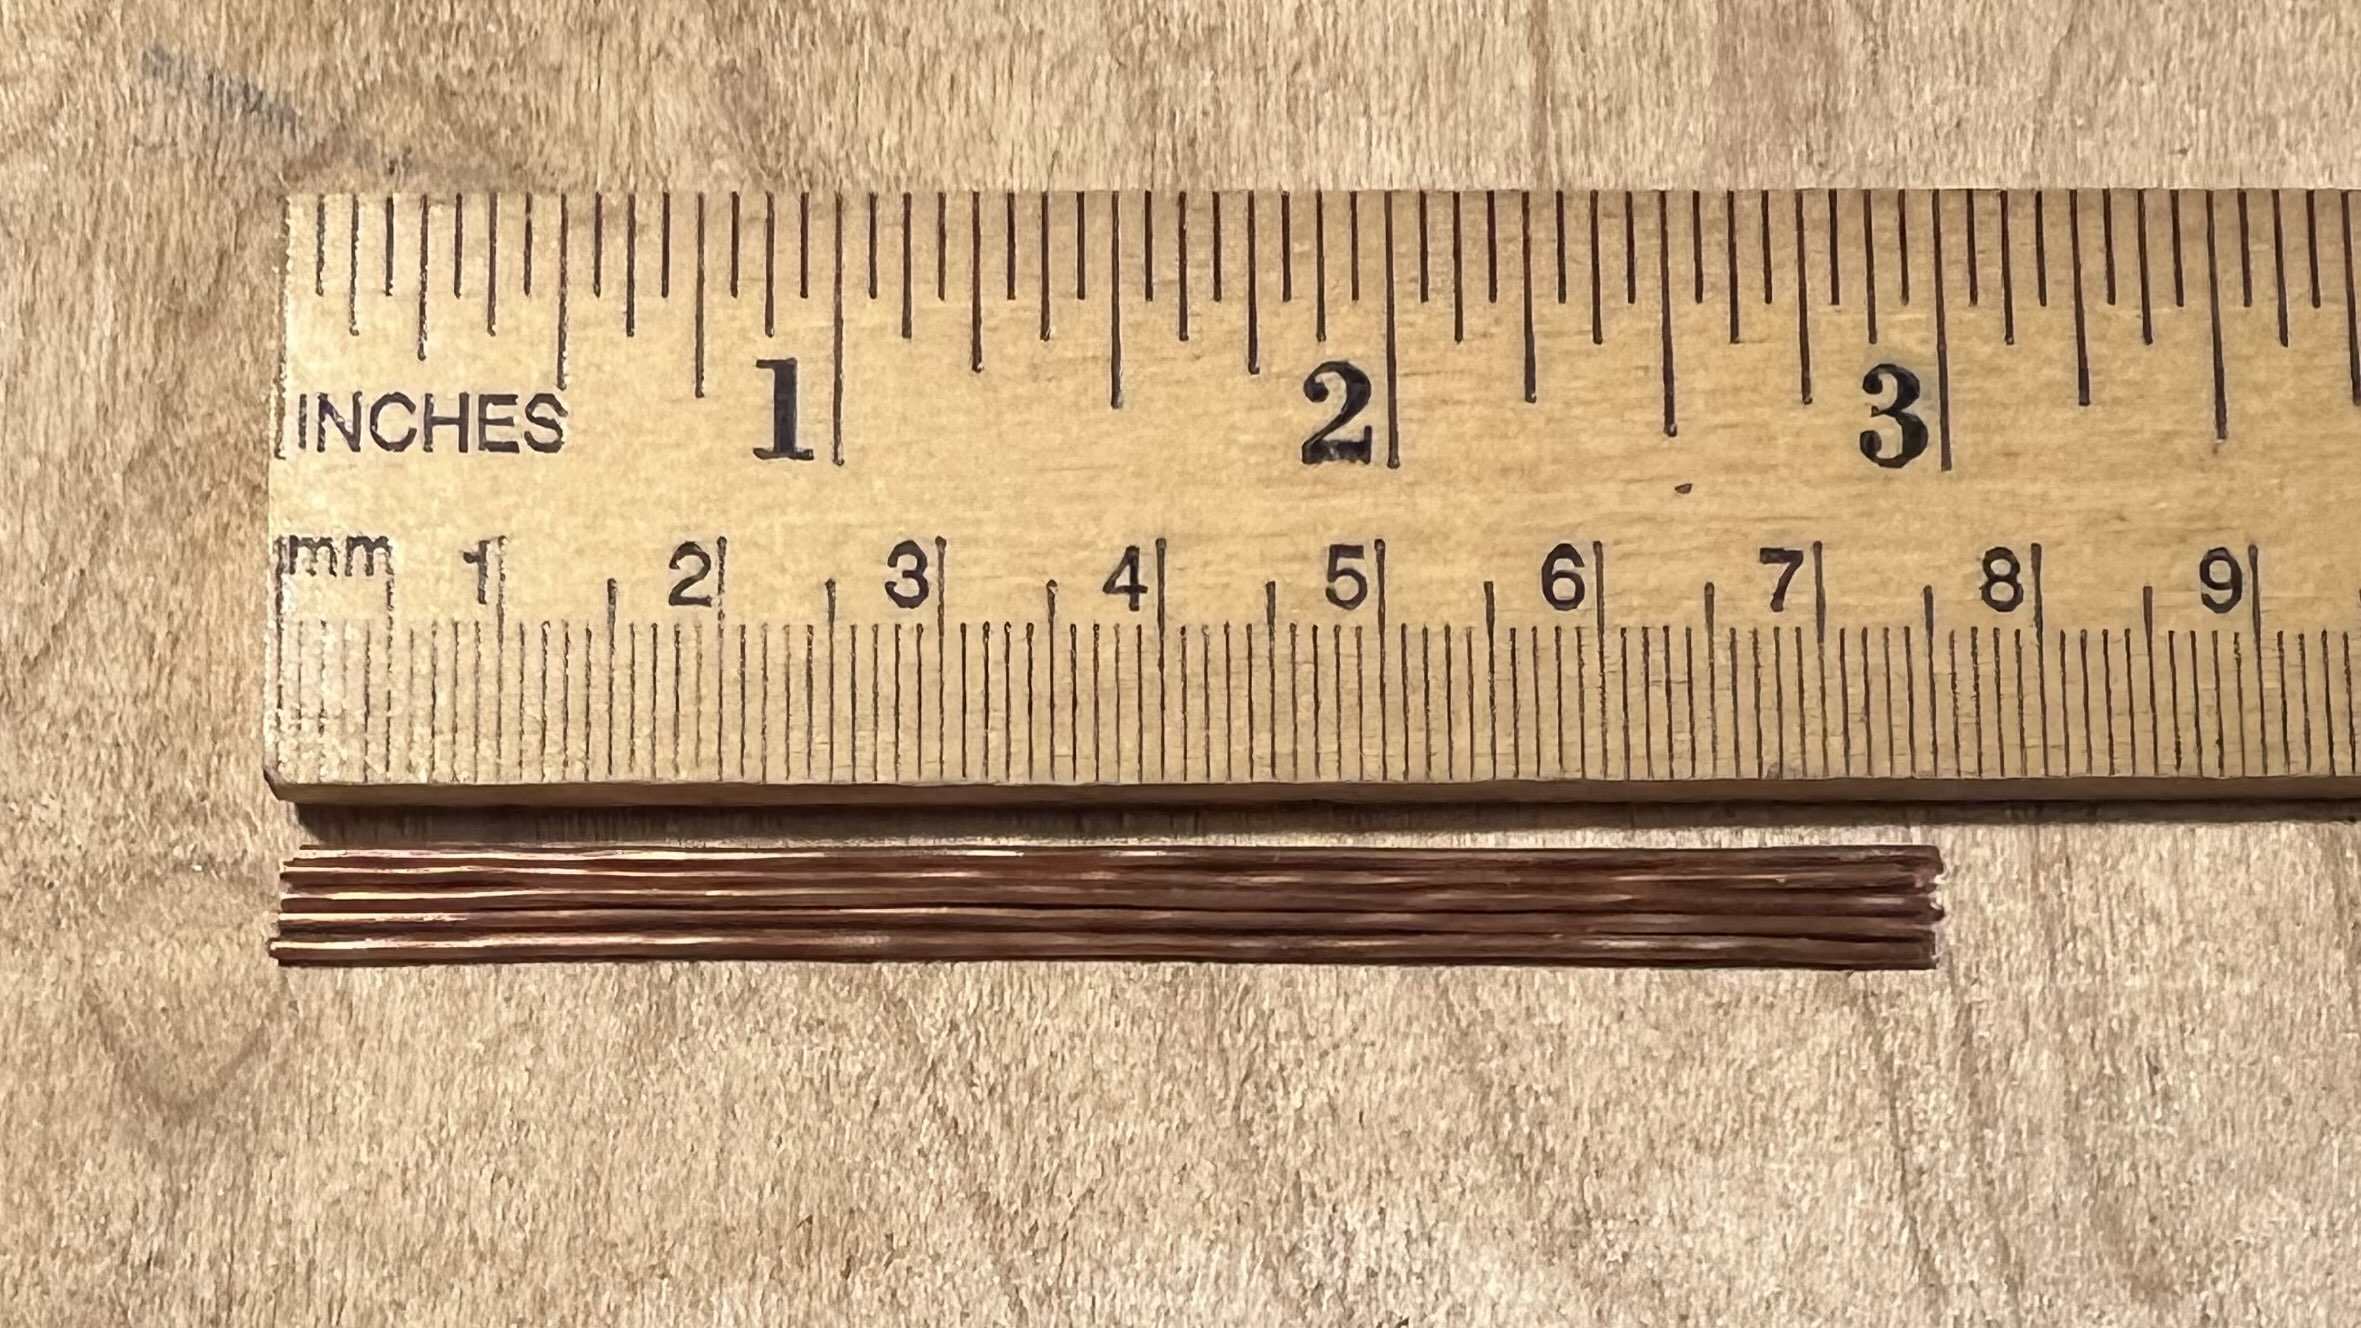
\includegraphics[width=0.5\textwidth]{./figures/fig_antenna elements straight.jpg}
  \end{center}
  \caption{75mm cut wires for antenna}\label{fig:ant_el_st}
\end{figure}

After the wires had been cut and straightened, four of them were bent at 135 degree angle approximately 3mm from the end. The four bent elements were soldered onto the four ground legs of the SMA connector, so that they are angled outwards and spaced 90 degrees apart in the XY plane. Next the remaining element was soldered onto the center pin of the SMA connector to complete the basic antenna design. 

\begin{figure}
  \begin{center}
    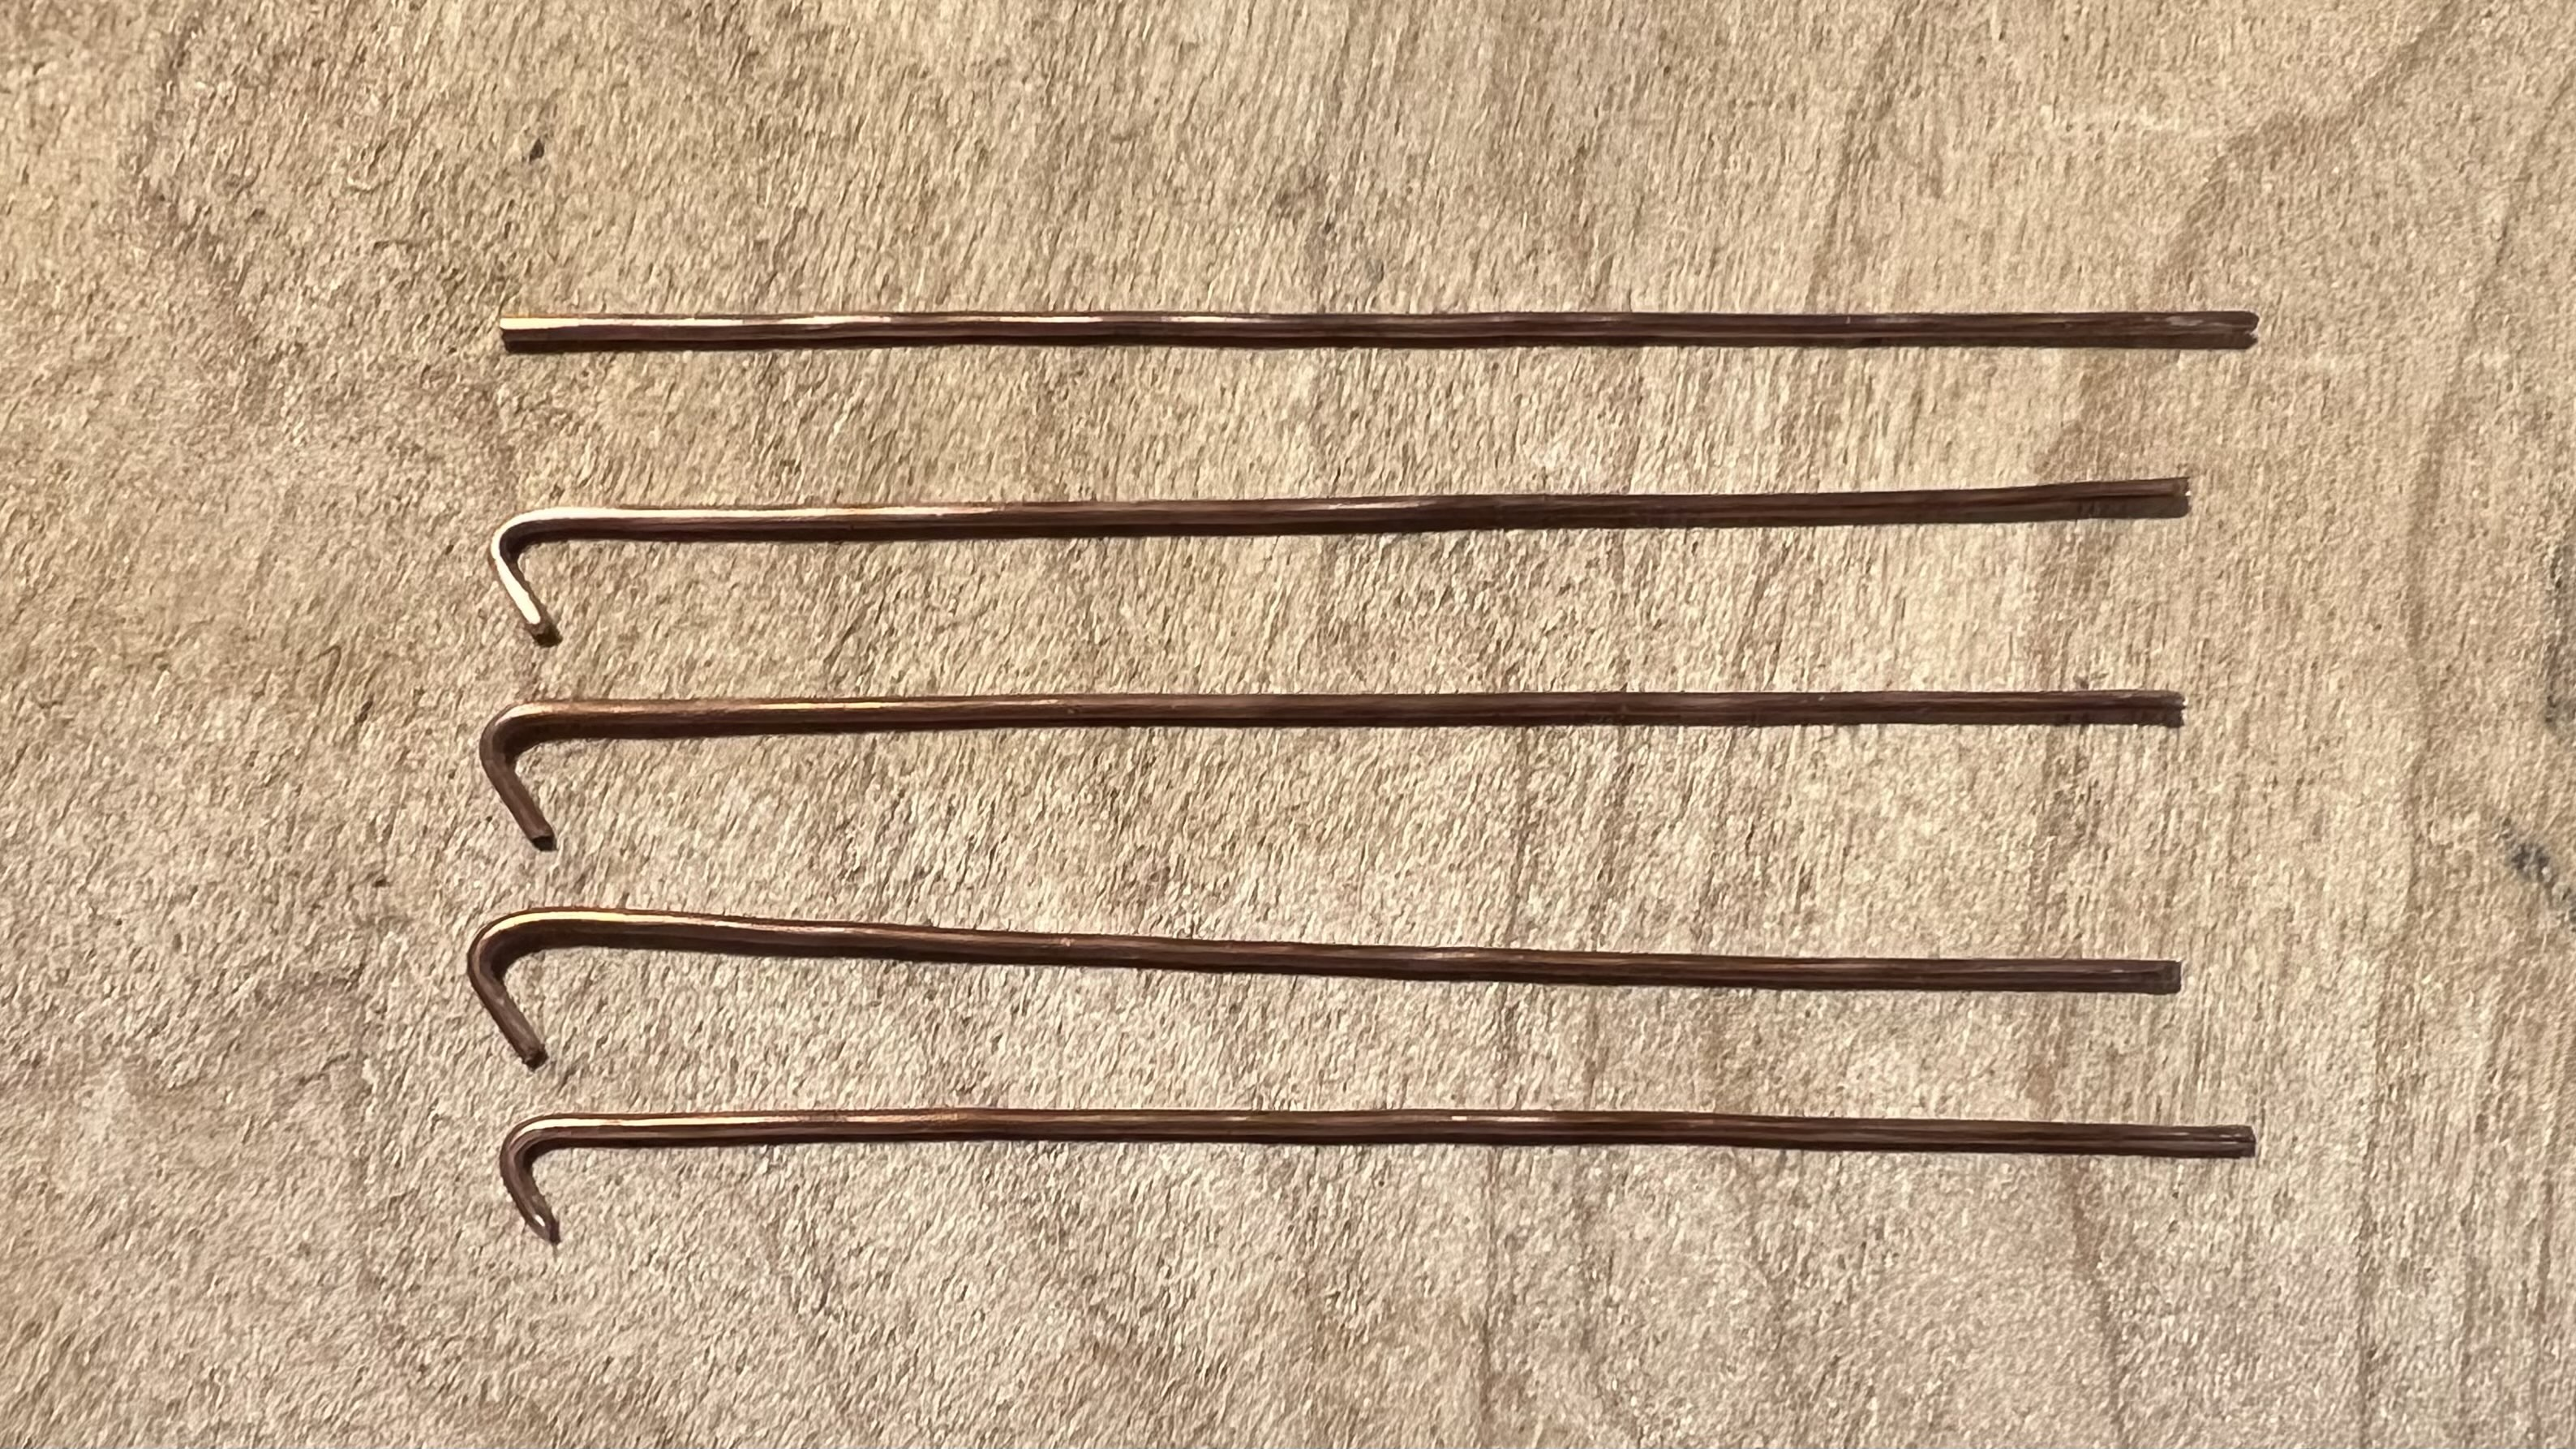
\includegraphics[width=0.5\textwidth]{./figures/fig_antenna elements-2.jpg}
  \end{center}
  \caption{Bent and straight elements for antenna construction}\label{fig:ant_el_bt}
\end{figure}

To test and tune the antenna, it was connected to a vector network analyzer (VNA), which would sweep a wide range of frequencies and measure the reflections of antenna. Initially, it showed the antenna having minimized reflections at around 900MHz, indicating that the elements were too long for optimal performance at 1090MHz. We then trimmed the elements slightly and retested in order to inch closer to our desired frequency, finally ending up with a return loss of $-40.6$dB and an input impedance of $49.1+0.221j\Omega$ at 1090MHz. These results were excellent, and the low mismatch between $49.1+0.221j\Omega$ and $50\Omega$ would result in minimal losses in the received signal.

\begin{figure}
  \begin{center}
    \includegraphics[width=0.5\textwidth]{./figures/fig_antenna_meas.jpg}
  \end{center}
  \caption{Antenna measurement with VNA}\label{fig:ant_meas}
\end{figure}

\begin{figure}
  \begin{center}
    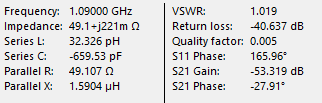
\includegraphics[width=0.5\textwidth]{./figures/fig_antenna_data.png}
  \end{center}
  \caption{Antenna properties at 1090MHz}\label{fig:ant_data}
\end{figure}

\begin{figure}
  \begin{center}
    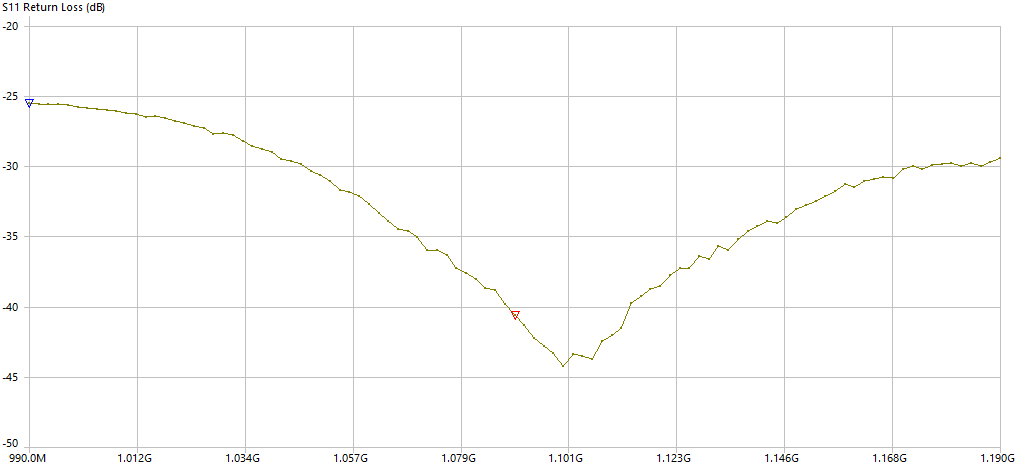
\includegraphics[width=0.5\textwidth]{./figures/fig_antenna_plot.png}
  \end{center}
  \caption{Antenna return loss plot}\label{fig:ant_plot}
\end{figure}

%% Matlab Implementation
\subsection{Matlab Implementation}
 Using \cite{matlabAir} we created a working output that was able to read some mock data for an ADS-B transmissions. In addition to helping us verify the ability to work with ADS-B signals in MATLAB, we were able to see how data is interpreted using an approach in code. However, the example given in the code was not useful in out manual implementation due to a lack of however level detail on ADS-B packet interpretation.

%% Out of Tree Modules for GNURadio
\subsection{Out of Tree Modules for GNURadio}
Another approach that we decided to implement was the use of an out-out-tree (OOT) module \cite{oot-adsb} in GNURadio. To our surprise, there was already a GNURadio module available to help interpret received signals using the given framing, demodulating, and decoding, blocks given in the `gr-adsb` package. From the example given in the repository for the OOT module shown in \autoref{fig:gr-adsb-example}, we can see that there are ADS-B Framer and ADS-B Demodulator blocks provided by the `gr-ads-b` OOT module. 

\begin{figure}
  \begin{center}
    % 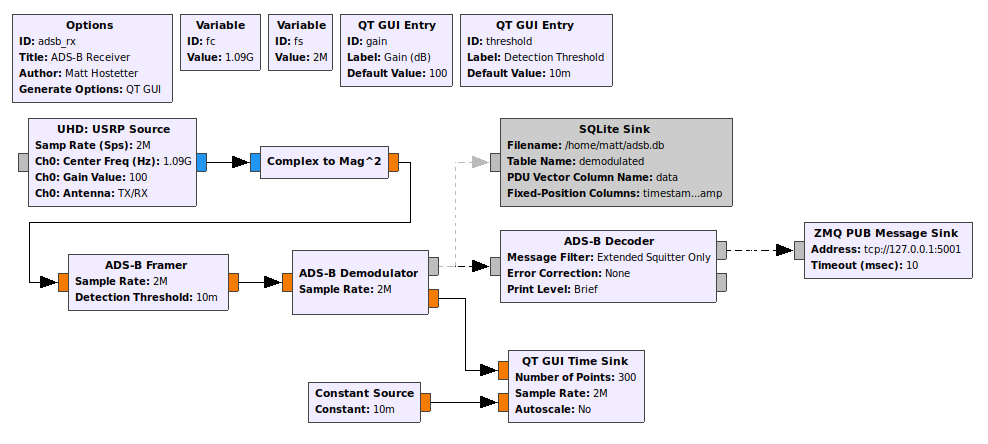
\includegraphics[width=1\textwidth]{./figures/adsb_rx.png}
    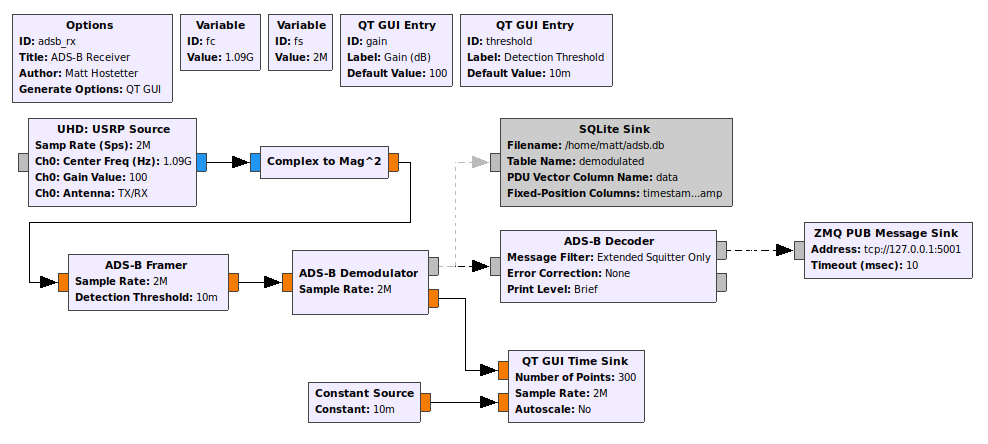
\includegraphics[width=\textwidth]{./figures/adsb_rx.png}
  \end{center}
  \caption{A GNURadio signal flow graph that is given as an example in the git repo where the `gr-adsb` module is available.}\label{fig:gr-adsb-example}
\end{figure}

However, after multiple attempts trying to install the package on an arch-linux based system, python package management was not allowing us to work with the manually installed packages for the `gnuradio.adsb` python modules. Regardless, we spent a bit of time looking at the source code of each of the modules to see how we would be able to implement similar function using individual blocks in GNURadio that are part of the Core package within GNURadio.

%% GNURadio Signal Flow Graphs
\subsection{GNURadio Signal Flow Graphs}
Implementing the actual communication protocol stack in GNURadio was done by using blocks that are part of the core library. An explanation of the pipeline is given below. First, we opened a connection to the PlutoSDR using the `PlutoSDR Source` block. The Pluto ran at a sample rate of 12MHz centered about 1090MHz. RF and DC correction was enabled in addition to quadrature sampling. Following the Pluto block was a rational resampler block that was used to help us debug different sample rates and decimation factors to receive a message at that correct frequency. After the rational resampler, there was a complex number to magnitude squared to convert the complex number into a float value that was captured. A gain block was used to boost the received signal after it has been converted to a float value. From there, the signal flow graph breaks out into two blocks, first a GUI time sink that was used to view the actual signal that has been received. Second, a threshold block that digitizes the data, we experimented with the values for the low and high threshold values to find the digitization scheme that rendered the best results. After the threshold block, there is another GUI time sink to view the digitized data in comparison to the non-digitized data. We also used a Correlate Access Code - Tag block to only allow signals that have the preamble within them to filter out non ADS-B signals. In cases where we wanted to use the signals that were passed through the Correlate Access Code - Tag block, we used a file sink that GNURadio writes to as a binary. A program was written in to read the data and decode the data.

\begin{figure}
  \begin{center}
    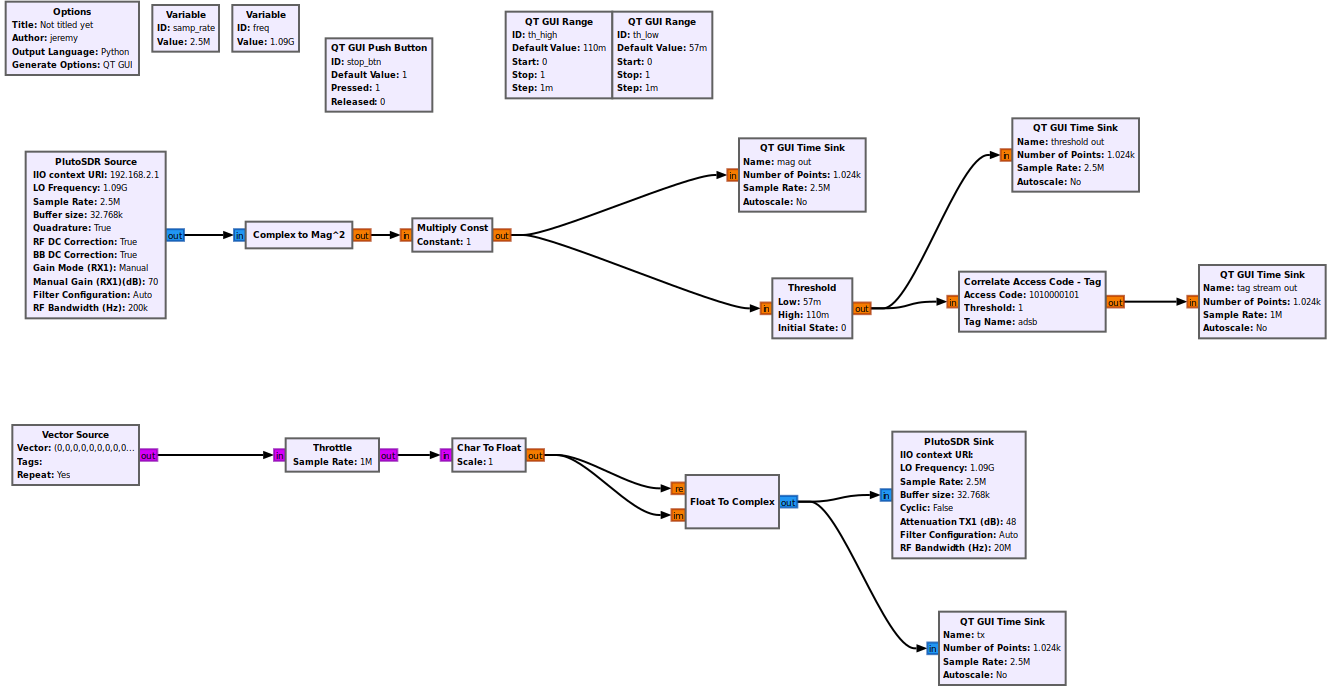
\includegraphics[width=\textwidth]{./figures/fig_gnuradio_loopback_test.png}
  \end{center}
  \caption{Signal Flowgraph for loopback testing of a simulated signal}\label{fig:loopback_grc}
\end{figure}

\begin{figure}
  \begin{center}
    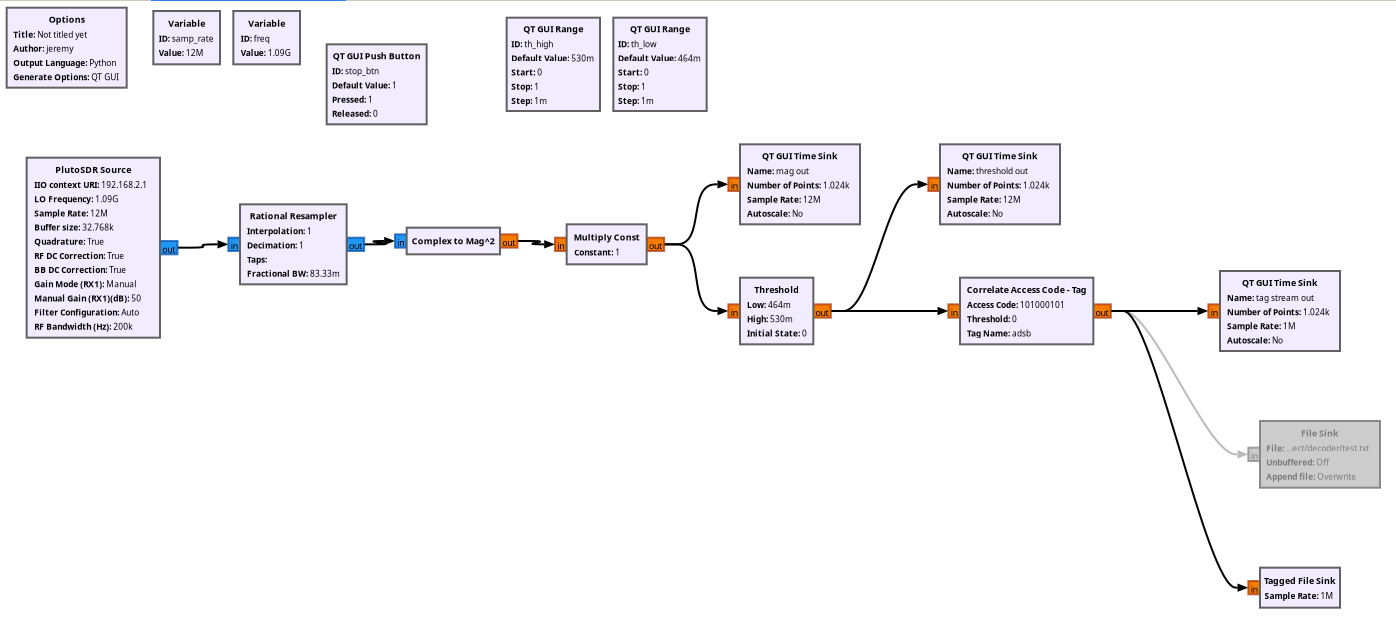
\includegraphics[width=\textwidth]{./figures/fig_sfg_gnuradio.png}
  \end{center}
  \caption{A screenshot of the signal flow graph used to receive messages from an aircraft.}\label{fig:fig_sfg_gnuradio}
\end{figure}


\section{Decoding the Data}
GNURadio writes data as a binary file when using the data sink, as such, we implemented the use of a C++ program to allow us to view and interpret the data. A program for opening and reading the data was made readily available on the GNURadio wiki page \cite{gnuradio-reading-file-cpp}. The program uses the fmt library\cite{fmt-library} to display error messages. After ensuring that the program was able to compile we wrote additional code to decode the received packet's position as shown in \autoref{fig:decode-position-adbs}. As you can see, the output decoded from a packet that we tested as shown in \autoref{fig:decode-position-adbs} gives a latitude and longitude.


\begin{figure}
  \begin{center}
    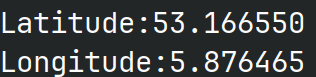
\includegraphics[width=0.3\textwidth]{./figures/fig_output_decode.png}
  \end{center}
  \caption{A screenshot of the longitude and latitude of a sample packet.}\label{fig:decode-position-adbs}
\end{figure}


%% Procedure
\section{Testing Procedure}
To conduct testing for our generated signal flow graphs, we took our Pluto modules outside of the Electrical and Computer Engineering building at the University of Arizona and began looking for signals that matched the ADS-B protocol. In addition to listening at the University of Arizona, one of the members of our team lives near the airport, so we were able to listen to signals there as well. We experimented with multiple gain values, digitization schemes, and error values for the ADS-B message preambles. After spending a cumulative total of a few hours we went back inside to examine the data.

\begin{figure}
  \begin{center}
    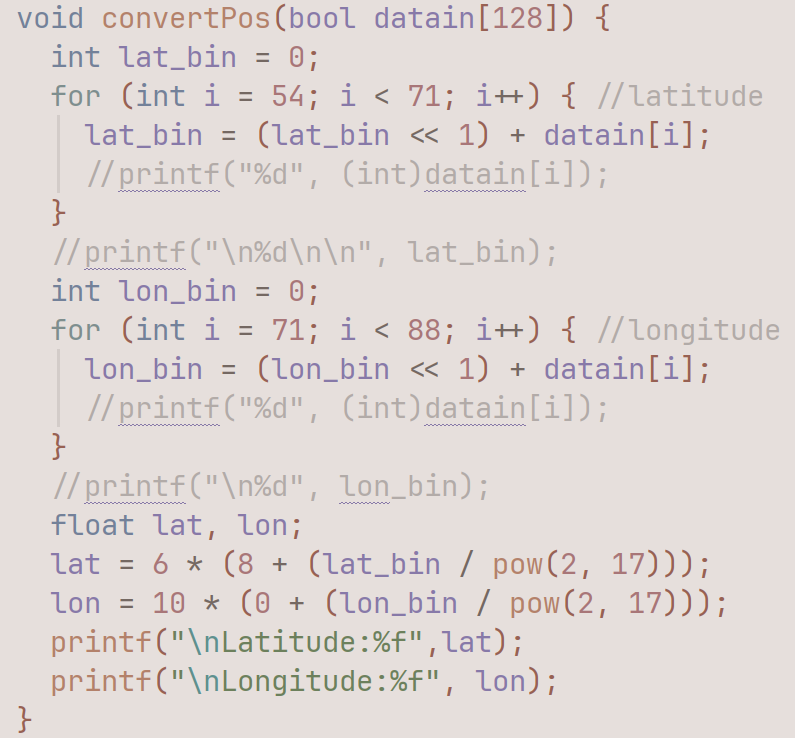
\includegraphics[width=0.5\textwidth]{./figures/fig_decode_position.png}
  \end{center}
  \caption{A screenshot of the code used to examine the position of the airplane sending the ADB-S packet.}\label{fig:decode-position-adbs}
\end{figure}

\begin{figure}
  \begin{center}
    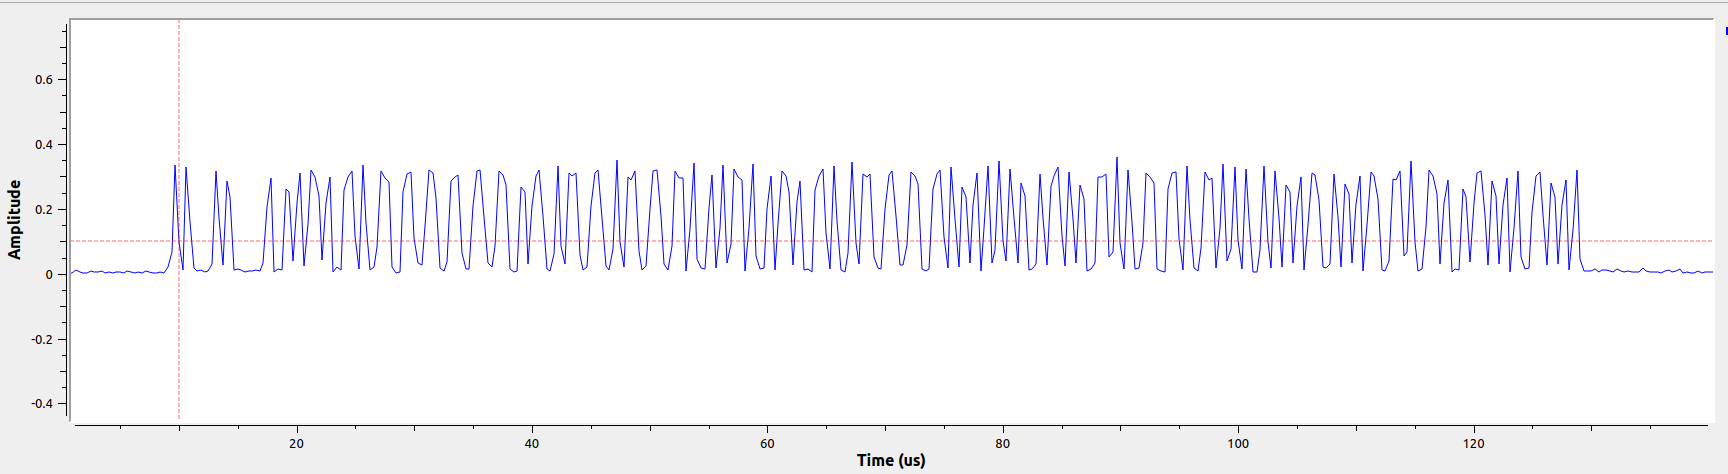
\includegraphics[width=0.5\textwidth]{./figures/fig_ADSB_recv_analog.png}
  \end{center}
  \caption{Analog ADS-B signal received by SDR}\label{fig:analog_rec}
\end{figure}

\section{Decoding the Data}
GNURadio writes data as a binary file when using the data sink, as such, we implemented the use of a C++ program to allow us to view and interpret the data. A program for opening and reading the data was made readily available on the GNURadio wiki page \cite{gnuradio-reading-file-cpp}. The program uses the fmt library\cite{fmt-library} to display error messages. After ensuring that the program was able to compile we wrote additional code to decode the received packet's position as shown in \autoref{fig:decode-position-adbs}.

\begin{figure}
  \begin{center}
    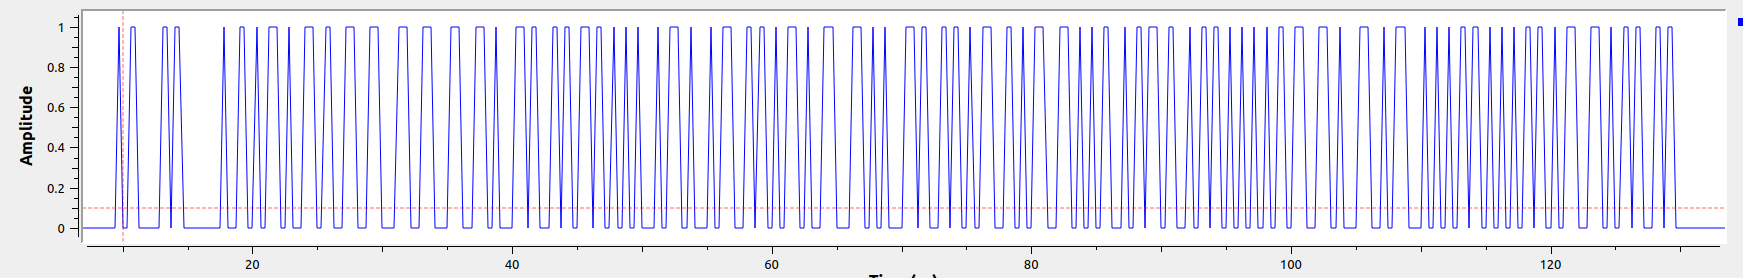
\includegraphics[width=0.5\textwidth]{./figures/fig_ADSB_recv_digital.png}
  \end{center}
  \caption{Digitized ADS-B signal from SDR}\label{fig:digital}
\end{figure}

\begin{figure}
  \begin{center}
    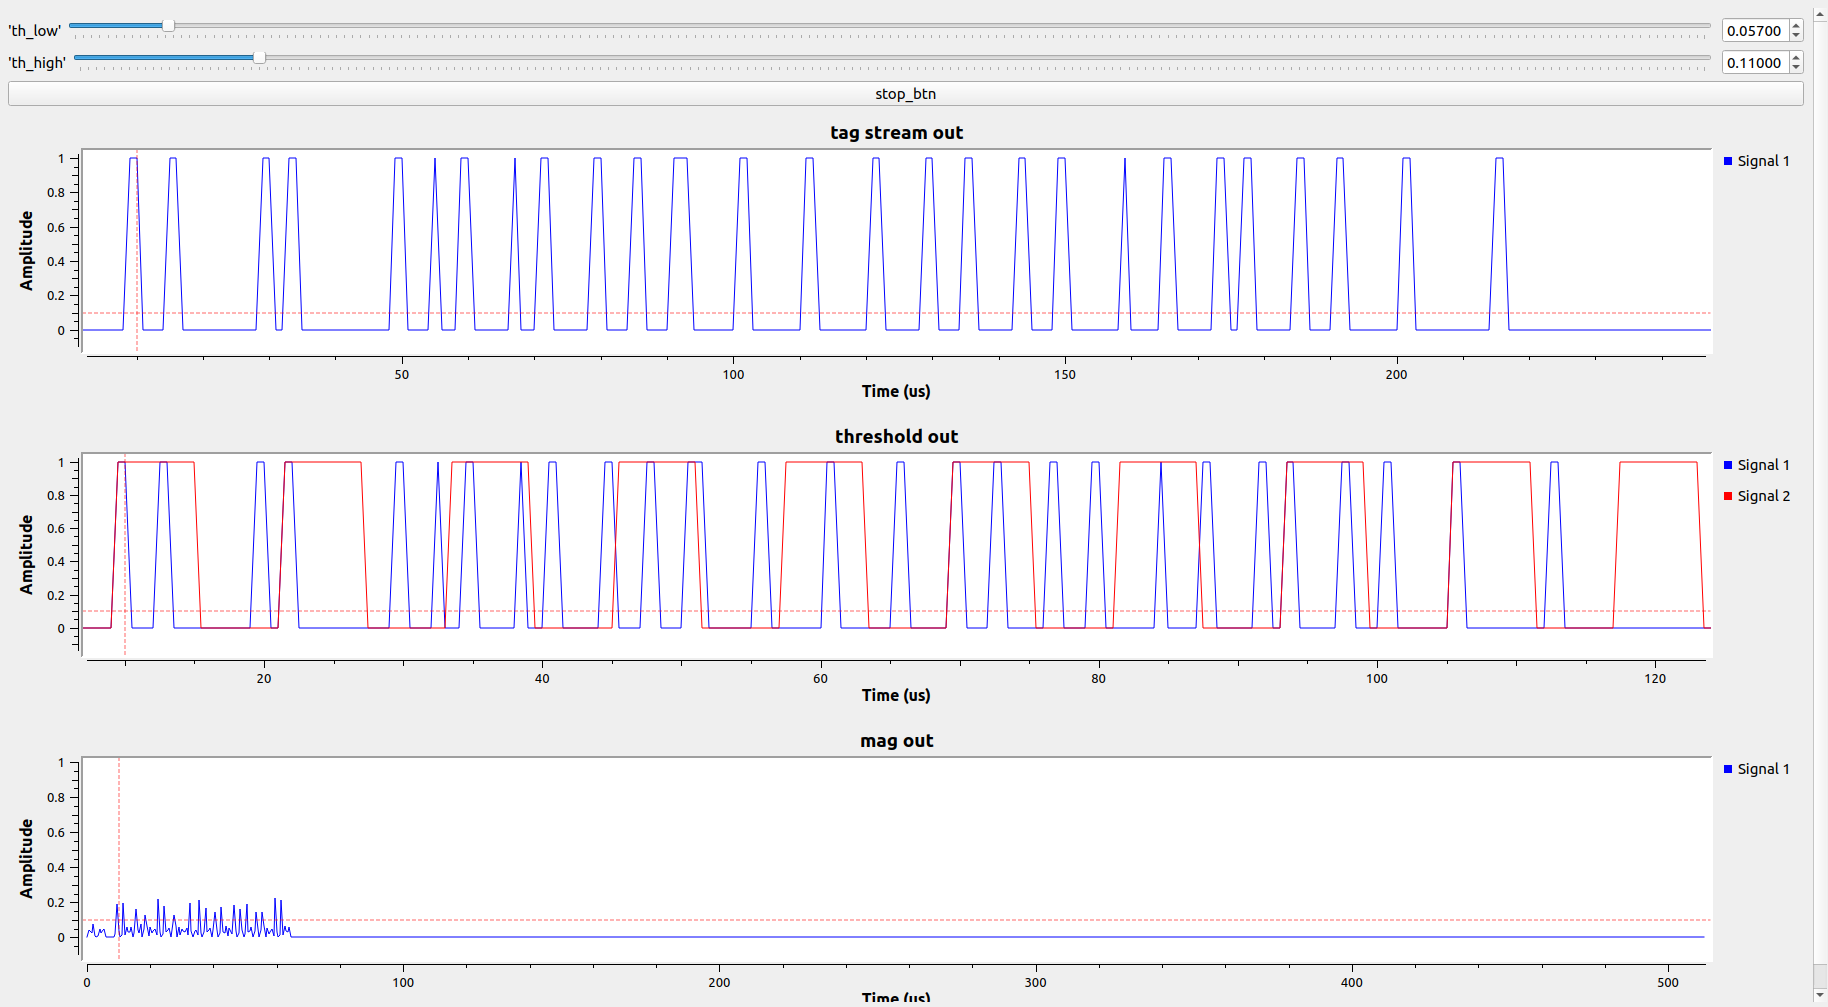
\includegraphics[width=0.5\textwidth]{./figures/fig_gnuradio_fullUI.png}
  \end{center}
  \caption{GNURadio UI used for adjusting digitization settings}\label{fig:receive_UI}
\end{figure}


%% Results
\section{Results}
After having run through our implementation and procedure, we ended up having mixed results on our project. Running the implementation provided by MATLAB showed us that ADS-S packets could be interpreted in MATLAB, but this was not useful to us. The examples given to us in the OOT `gr-adsb` module did not work on our system due to package management issues in Python. Our GNURadio signal flow graphs did accomplish different parts of the experiment, however, we were unable to combine multiple parts of the signal flow graphs to accomplish all of the tasks in an automated way. While we were able to successfully receive signals that were being sent in the 1090MHz range, we were unable to use the Correlate Access Code block to successfully filter out only the signals that were actual ADS-B signals. As you may have noticed, we used a sample packet that we created to check if our decoder scheme was correct in out C++ implementation. This is because files that GNURadio wrote to an output were too large for us to use/filter through, as such, we created a sample packet to verify that our decoder worked. Luckily, the decoder did work. (after filtering out the preamble.) When using the file sink in GNURadio, we ran into the problem of too much data being recorded, this led to file sizes that were too large to work with. We tried to implement logic in GNURadio to only write to a file when a signal gets filtered through the Correlate Access Block, however, there were issues with that. One part of the experiment that was very successful was the custom antenna that we made to make sure that the SNR was sufficient to give us enough 'room' to raise the gain and receive signals at the University. This benefit was noticed when trying to receive signals using the antennas that came with the Pluto in comparison to the custom antenna we made. Funnily enough, the custom antenna was not needed when receiving signals next to the airport.


%% Problems with Frame Synchronization
\section{Error Analysis}
During testing we noticed that there was a mismatch between the sample rate and data rate. Our data processing required one sample per data bit at 1MHz, however our sample rate had to be significantly higher to account for small variations in the analog signal. To try and account for this mismatch, we tried using a resampler block with the proper ratio to downsample the signal. Unfortunately, this had the issue of shortening and lengthening some of the data bits when they were slightly out of sync with the lower sample rate, thus making the data incompatible with our data processing algorithm.

The beginning of an ADS-B frame consists 16 bits that make up the preamble of the frame. These 16 bits can be used to synchronize the beginning of the frame and mark the following data as a usable signal using the Correlate Access Code-Tag block. With the aforementioned bit width issue, the preamble data was not consistent and could not be properly synchronized at the beginning of the frame. We then attempted to increase the number of allowable errors in the preamble, but this did not solve the issue as all of the data was too inconsistent.


%% Conclusion
\section{Conclusion}
Throughout this project, we had many interesting experiences that challenged our abilities in GNURadio. Attempting to build an ADS-B reciever allowed us to explore many tangential aspects of using a software defined radio, such as antenna design, antenna construction, data processing, and dealing with large quantites of binary data. While this project was not completely successful from a technical perspective, largely due to our difficulties in frame synchronization, it was very successful from an educational standpoint. We learned to apply digital signal processing concepts as well as communication theory to transmit test signals between SDRs and interpret afformentioned test signals. Overall we learned a significant amount from this project and have a newfound respect for radio engineers.



%% Generate the BibTeX bibliography.
\bibliographystyle{ieeetr}
\bibliography{refs}

\end{document}

